\section{Related Work}

\begin{figure*}[t]
\centering
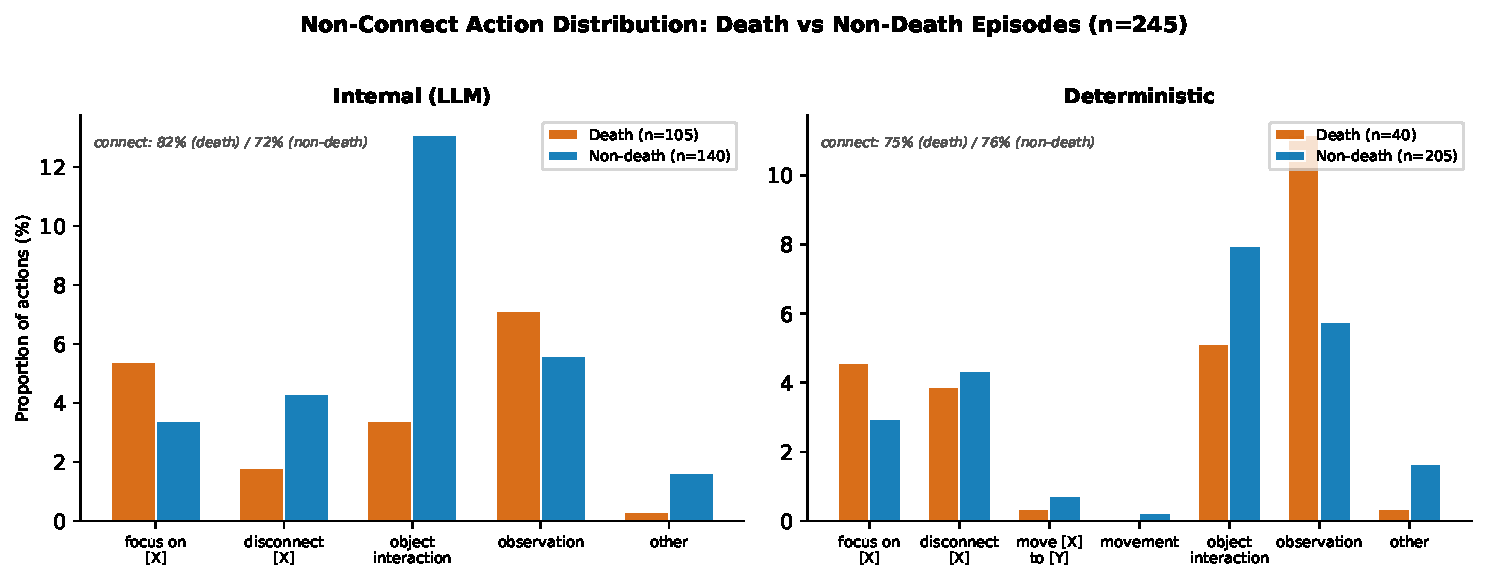
\includegraphics[width=\textwidth]{figures/death_action_comparison.pdf}
\vspace{-2mm}
\caption{Non-\texttt{connect} action distribution comparison between internal (left) and deterministic (right) strategies within death episodes. Both strategies exhibit comparable \texttt{focus on} rates (${\sim}5\%$); the internal strategy's higher death count (105 vs.\ 40) reflects more frequent entry into catastrophic states, not different action selection within those states.}
\label{fig:death-comparison}
\end{figure*}

\paragraph{Tool-Augmented Agents and Adaptive Routing.}
Methods for augmenting LLMs with external tools span self-supervised invocation~\citep{toolformer-2023,toolace-2025}, task-level decomposition~\citep{art-2023,chameleon-2023}, and RL-based tool selection~\citep{retool-2025,tool-learning-survey-2024}. Concurrent work examines \emph{when} to invoke tools: \citet{when2tool-2026} analyze accuracy--latency tradeoffs, \citet{tool-use-tax-2026} quantify invocation overhead, and \citet{to-call-or-not-2026,tool-overuse-illusion-2026} investigate overuse patterns. On the routing side, adaptive methods range from learned halting~\citep{graves2016act} and token-level recursion~\citep{mixture-of-recursions-2025} to per-step depth adjustment~\citep{cogrouter-2026,ares-2026} and multi-turn model selection~\citep{mtrouter-2026}. Model-selection routing~\citep{routellm-2024,frugalgpt-2023,automix-2024} optimizes \emph{which} model to invoke based on query difficulty; \citet{budget-aware-routing-2026} train episode-level routing under sparse rewards via counterfactual rollouts, the closest setting to ours, though they focus on learning the router rather than diagnosing what signal it captures. All these approaches presuppose that diverse routing signals exist; our decomposition reveals that in ScienceWorld, a single mechanism accounts for 78.9\% of routing labels.

\paragraph{Counterfactual Methods and Agent Environments.}
Prior work generates counterfactual explanations by perturbing individual actions~\citep{olson2021counterfactual,gajcin2023counterfactual,amitai2024explaining}; recent extensions target LLM agents via abstract state comparison~\citep{pona2025abstract}, axis-aligned perturbations~\citep{axis-2026}, and causal structure discovery~\citep{cso-2026}. These approaches explain \emph{why} an agent succeeded or failed on a single trajectory. We instead execute complete episodes under two strategies to decompose routing signal \emph{before} training. Counterfactual data augmentation~\citep{kaushik2020learning} edits inputs to improve robustness; we execute full counterfactual \emph{episodes} under controlled strategy variation, answering what \emph{type} of signal drives strategy preferences. ScienceWorld~\citep{scienceworld-2022} serves as our primary testbed; ALFWorld~\citep{alfworld-2021} and AgentBench~\citep{agentbench-2024} provide complementary evaluation. ReAct~\citep{react-2023} is our internal baseline; Reflexion~\citep{reflexion-2023} and LATS~\citep{lats-2024} extend it. The concurrent SALT~\citep{salt-2026} assigns step-level credit on ALFWorld, complementing our episode-level decomposition.

\paragraph{Safe RL, Agent Safety, and Causal Inference.}
Death avoidance connects to safe RL~\citep{garcia2015comprehensive,achiam2017cpo}, shielding~\citep{alshiekh2018safe}, and the growing literature on LLM agent safety evaluation~\citep{ruan2024failures,saferoute-2025,agent-safetybench-2024}. Classical safe RL methods require known transition dynamics or a differentiable safety model, neither available for black-box LLM agents. Unlike token-level adaptive computation~\citep{mixture-of-depths-2024,xin2020deebert} and mixture-of-experts routing~\citep{switch-transformer-2022}, which optimize compute allocation at inference time, our framework diagnoses aggregate routing signal at episode granularity. Methodologically, our pure-strategy comparison is a simplified potential outcomes framework~\citep{rubin1974estimating}: executing both strategies under identical initial conditions eliminates confounding without structural causal models~\citep{pearl2009causality}, at the cost of requiring paired episode collection.
